\subsection*{Human Interactome}

As the first step in the evaluation of A2, A3 and L3 methods for link
prediction, the full calculation and ranking of all predictions was
carried out. The results for the analyzed human interactomes (\emph{HI-II-14}
and \emph{HI-TESTED}) is shown in Figure \ref{fig:HI1}, in which
the x axis represents a rank position $k$ and the y axis displays
the precision for the top $k$ predictions of each method, when assuming
interactome \emph{HI-III} as the validation set. 

\begin{figure}[h]
\caption{\label{fig:HI1}Methods Comparison for \emph{HI-II-14} and \emph{HI-TESTED}}
	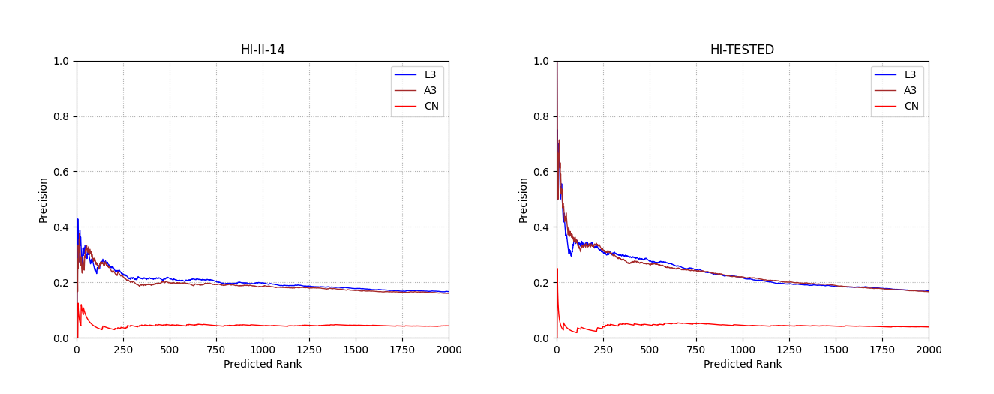
\includegraphics[width=\textwidth ]{figures/figure2.eps}
	%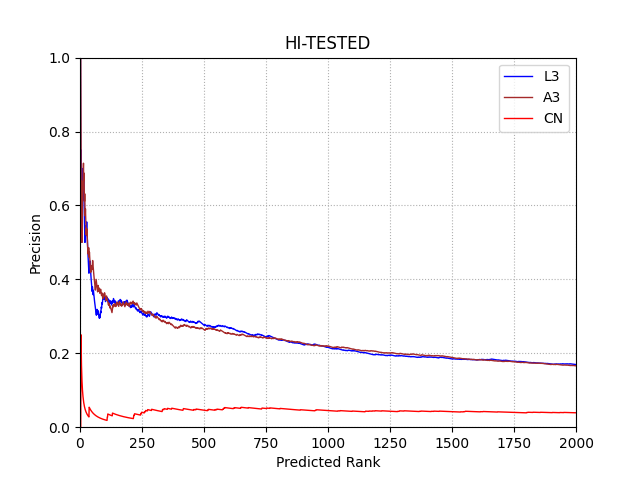
\includegraphics[width=0.7\textwidth ]{../hi-tested.txt.}
\end{figure}

As it can be inferred from the plots, L3-based predictions outperform
their $A{{}^2}$ counterparts. Results also show that L3-score and
$A^{3}$predictions follow a very similar trend.

However, it is of our interest to assess if Machine Learning can boost
the overall performance on the prediction, so the proposed procedure
was adapted to the human interactome data: Instead of having to remove
a fraction of edges from the network in order to predict and validate,
the prediction network and the validation networks are given beforehand.
The rest of the procedure is carried out as mentioned in Section 2.
Table \ref{T1} presents the results for the combinations of Node2Vec
with each feature.

\begin{table}
\caption{\label{T1}Summary statistics for human interactomes}
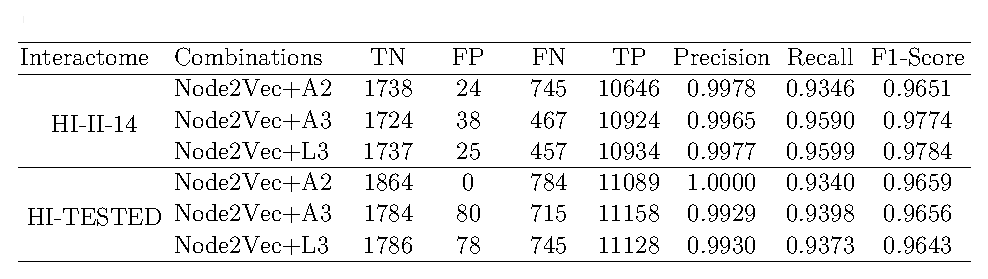
\includegraphics[width=1\columnwidth]{figures/T1}
\end{table}

In general, performance of all models is above 0.96 in terms of F1-Score.
Although marginally, the A2 feature-enriched model for HI-TESTED performs
better than their counterparts based on paths of length 3. The opposite
is also true for HI-II-14: models enriched with L3 and A3 features
perform better than their A2 counterpart. Results for the Interactome
\emph{HI-II-14} with Node2Vec and each metric are presented in Figures
S\ref{HI1}, S\ref{HI2} and S\ref{HI3}. It can be seen that for
\emph{HI-II-14}, A2 performs marginally better than L3 when comparing
precision but worse in terms of recall, although all metrics have
AUC values of 0.99.

On the other hand, the interactome \emph{HI-TESTED} was assessed with
the same methodology as \emph{HI-II-14} and results are shown in Figures
S\ref{HI1-1}, S\ref{HI2-1} and S\ref{HI3-1}. For this interactome,
A2 performs better in terms of false positives than A3 and L3, but
in terms of false negatives, A3 actually performs better that A2 and
L3. In terms of AUC, metrics results are indistinguishable. 

An interesting assessment from this human datasets can be observed
when looking at the importance plots, which show a very biased influence
of the handcrafted features. Figure \ref{F8-importance-H1} shows
this behavior for the \emph{HI-II-14} dataset, which is very similar
to \emph{HI-TESTED} (Figure S\ref{F8-importance-H2}).

\begin{figure}[h]
\noindent \begin{centering}
\caption{\label{F8-importance-H1}Importance gain plots for \emph{HI-II-14}}
\par\end{centering}
\begin{centering}
\includegraphics[width=0.48\columnwidth]{figures/Human/Imp\lyxdot A2\lyxdot 1\lyxdot eps}\includegraphics[width=0.48\columnwidth]{figures/Human/Imp\lyxdot A3\lyxdot 1\lyxdot eps}
\par\end{centering}
\centering{}\includegraphics[width=0.48\columnwidth]{figures/Human/Imp\lyxdot L3\lyxdot 1}
\end{figure}


\subsection*{Rice Interactome}

For the rice interactome, different combinations of features were
trained on the model and validated. The results are shown in Table
\ref{T2}. First, prediction based on \texttt{Node2Vec} without any
additional feature included is used as baseline of comparison. Figure
\ref{F1} shows those results, and one can see that its mean performance
using the AUC is $0.93$. The results for all 10 repetitions of each
model are consistent, meaning the variance among each line is not
significant. The results for each model using only the default features
are satisfactory. This result can also be assessed when looking at
the confusion matrix, where a precision of $0.98$ and a recall of
$0.86$ are obtained.

\begin{table}
\caption{\label{T2}Summary statistics for rice interactome}
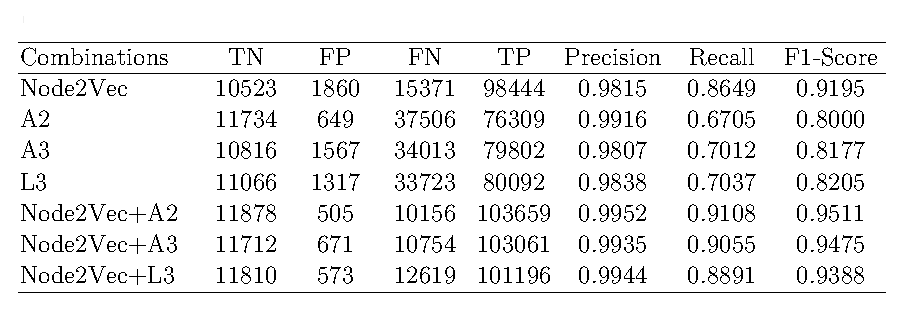
\includegraphics[width=1\columnwidth]{figures/T2.eps}
\end{table}

\begin{figure}[h]
\noindent \begin{centering}
\caption{\label{F1}Summary ROC curves for \texttt{Node2Vec} model alone}
\par\end{centering}
\noindent \raggedleft{}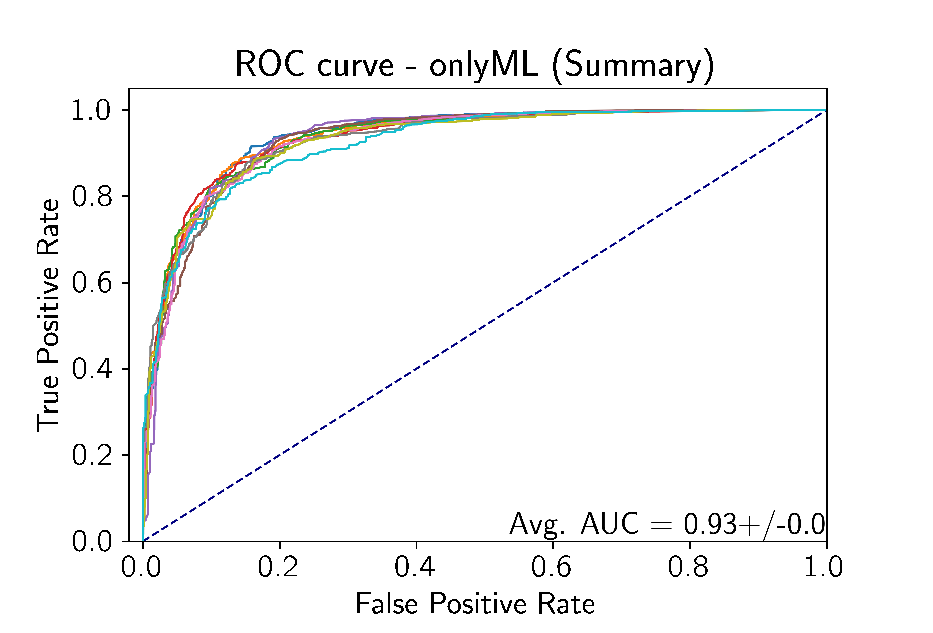
\includegraphics[width=0.48\columnwidth]{figures/Only_ML/ROConlyML_SUMMARY.eps}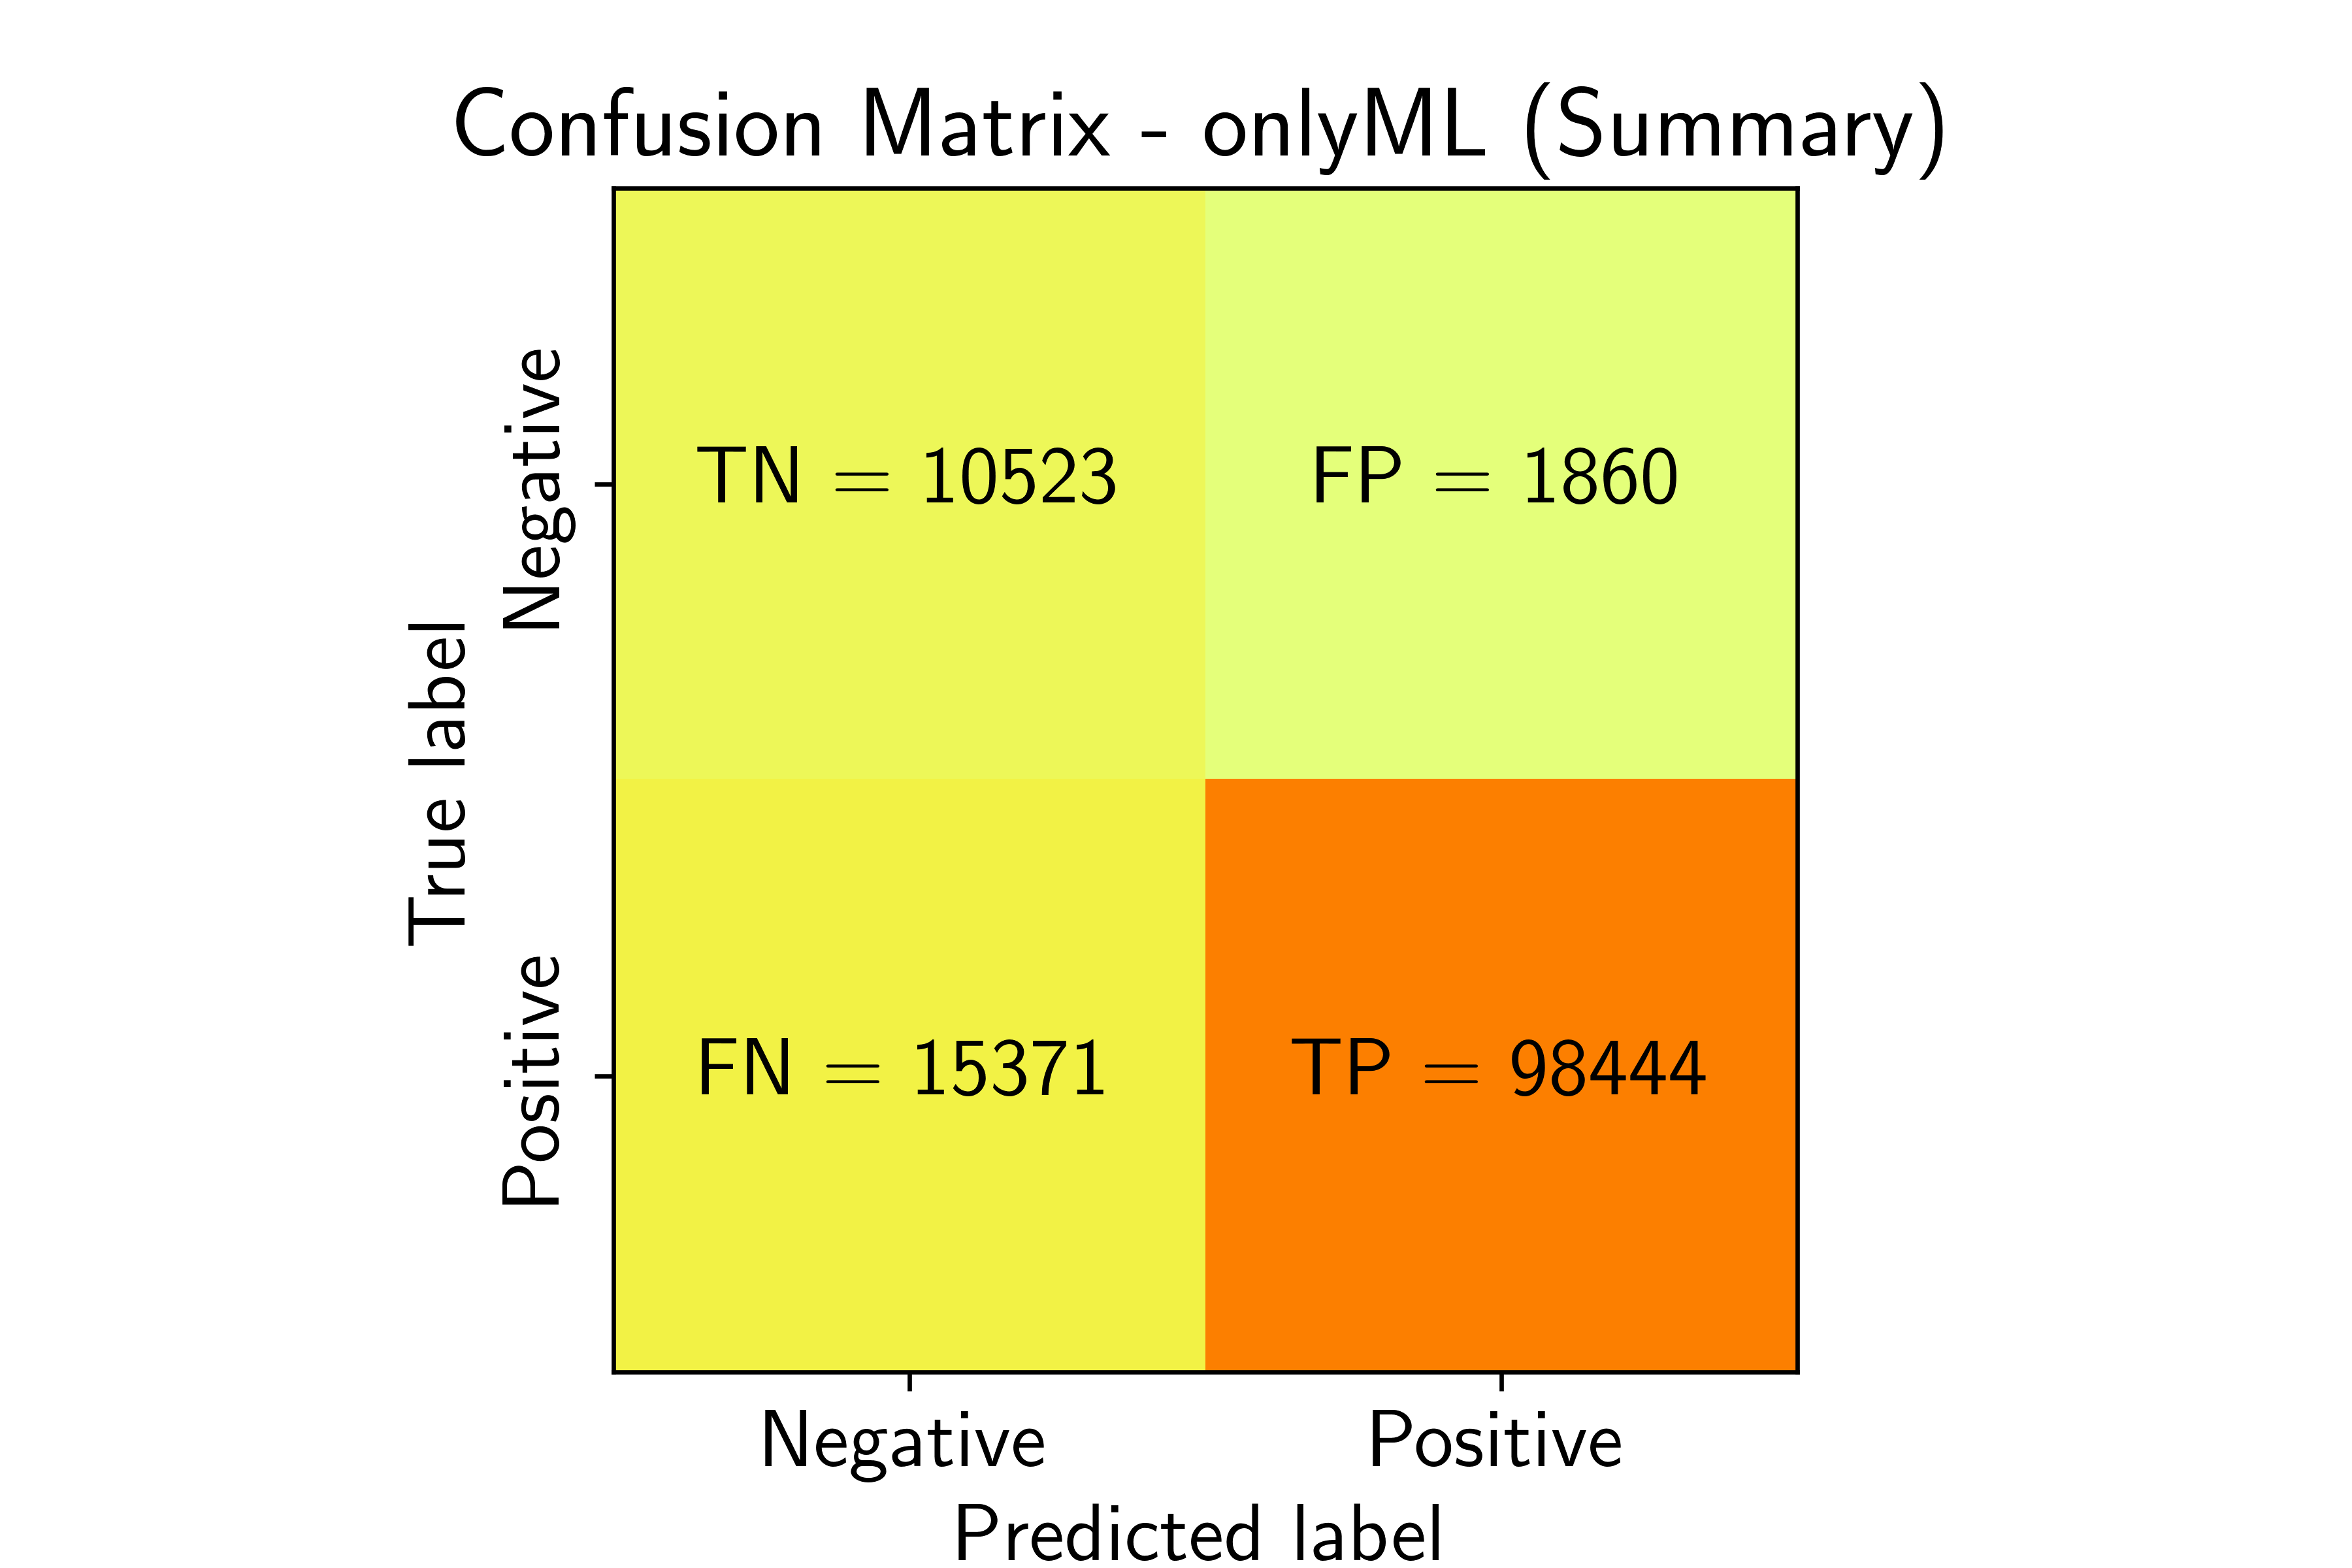
\includegraphics[width=0.48\columnwidth]{figures/Only_ML/CMonlyML_SUMMARY.eps}
\end{figure}

The next experiment carried out was to add for each prediction method
score as a prediction feature, that is, use the score as an additional
feature for the ML algorithm. Results for the Common Neighbors method
(\textbf{A2}), which uses paths of length 2, are shown in Figure S\ref{F2}.
All 10 experiments have small variability among them and perform better
than the baseline, with AUC of $0.98$. When looking at the confusion
matrix for this model, most guesses are true positives and true negatives,
resulting in a precision of $0.99$ and a recall of $0.91$. The same
analyses are done with the count of paths of length 3 (\textbf{A3})
and with the degree-normalized length-3 score (\textbf{L3}). These
results are presented in figures S\ref{F3} and \ref{F4}, respectively.
The corresponding AUC are $0.97$ and $0.98$.

\begin{figure}[h]
\noindent \begin{centering}
\caption{\label{F4}Results for \texttt{Node2Vec} with L3 feature}
\par\end{centering}
\noindent \raggedleft{}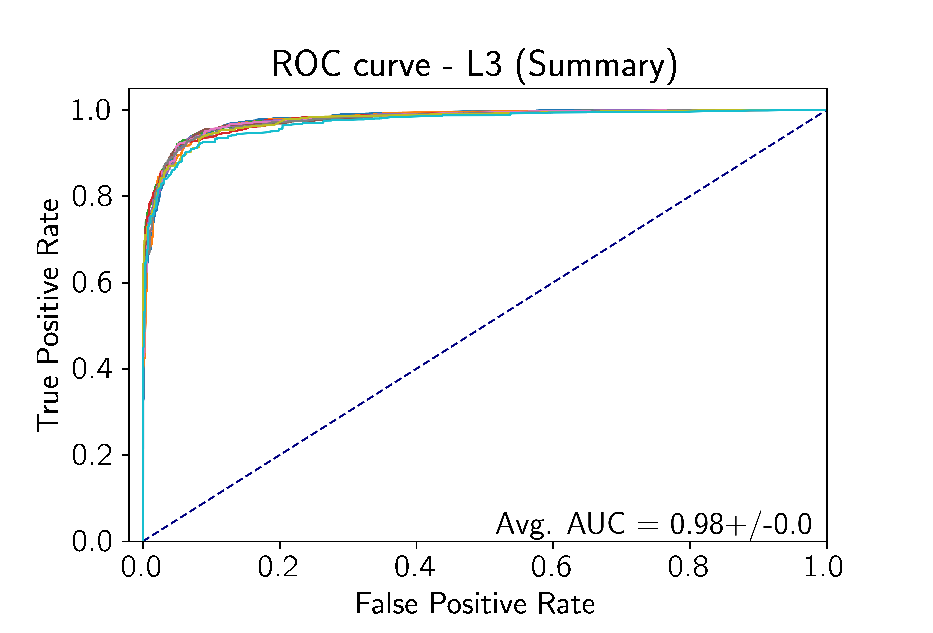
\includegraphics[width=0.48\columnwidth]{figures/ML_Metric/ROCL3_SUMMARY.eps}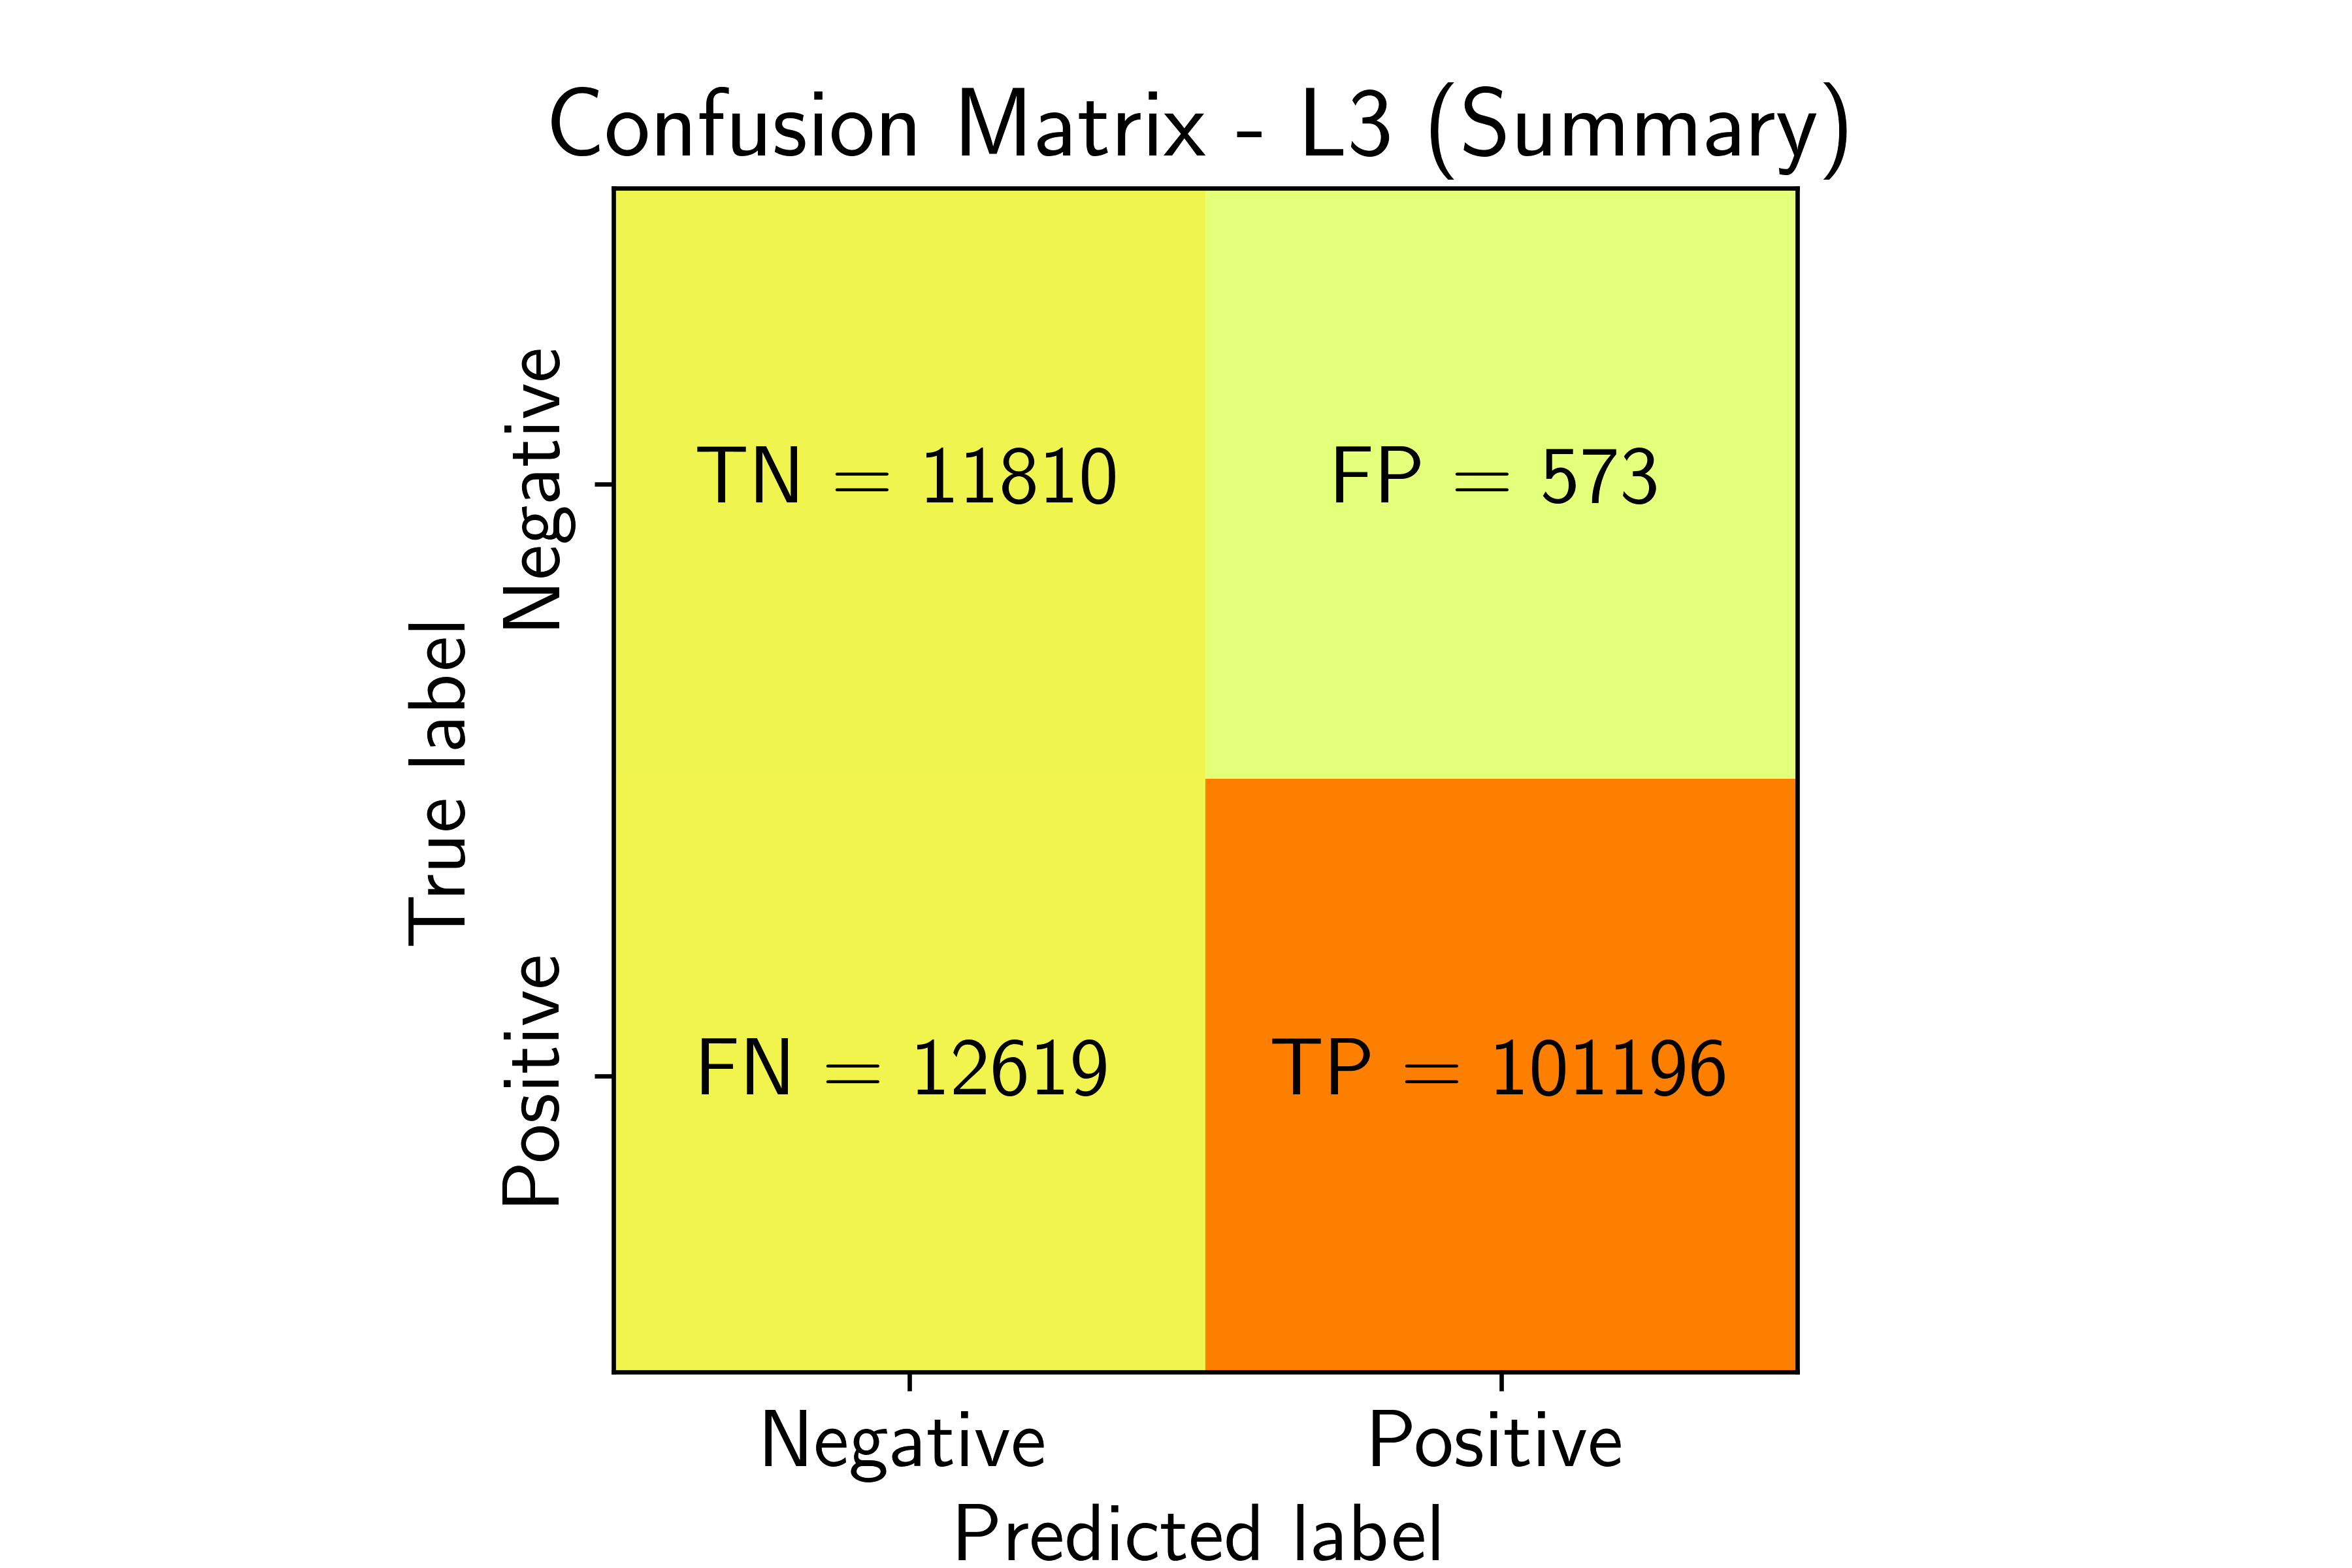
\includegraphics[width=0.48\columnwidth]{figures/ML_Metric/CML3_SUMMARY.eps}
\end{figure}

The precision when using the count of paths of length 3 (A3) is $0.99$
while the recall is $0.90$. It is interesting to observe that precision
decreased $0.16\%$ and recall decreased $0.58\%$. A similar situation
is obtained for the model with the normalized score (L3), whose precision
decreased to $0.99$ ($-0.08\%$) and recall decreased to $0.88$
($-2.38\%$). It can be seen also that the ROC curve achieves high
values of true positive rate sooner in the A2-featured model than
on the other models.

Another relevant assessment was carried out to verify the predictive
power of the metrics. \texttt{XGBoost} models were trained only using
each metric, for the same 10 experiments. Results are shown in Figures
S\ref{F5}, S\ref{F6} and \ref{F7}. XGBoost yields lower AUC values
when only considering A2, A3 and L3. Precision and recall for this
assessments, although lower than the previous experiments, are still
considered satisfactory.

\begin{figure}[h]
\noindent \begin{centering}
\caption{\label{F7}Results for L3 feature alone}
\par\end{centering}
\noindent \raggedleft{}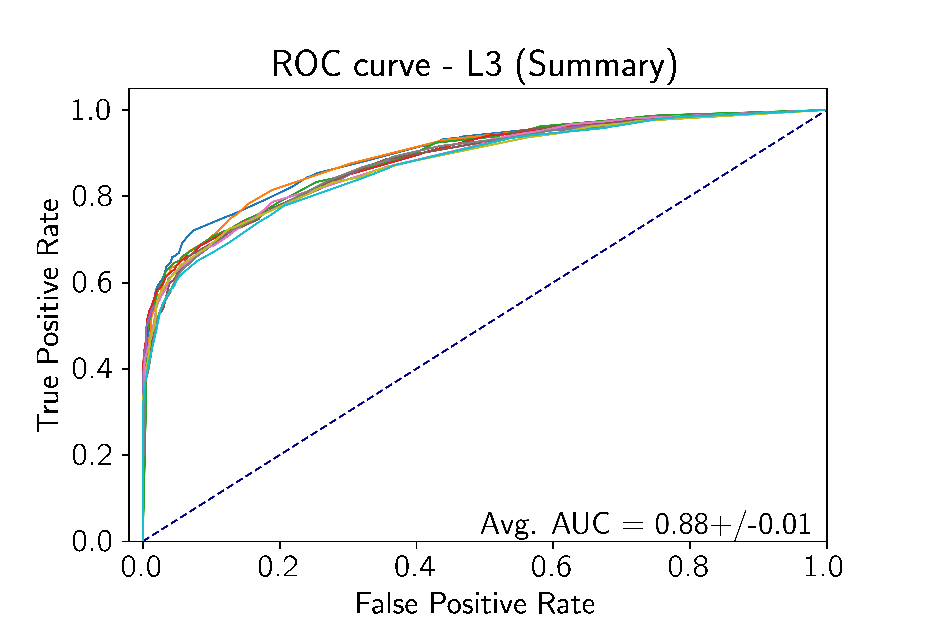
\includegraphics[width=0.48\columnwidth]{figures/Only_Metric/ROConlyL3_SUMMARY.eps}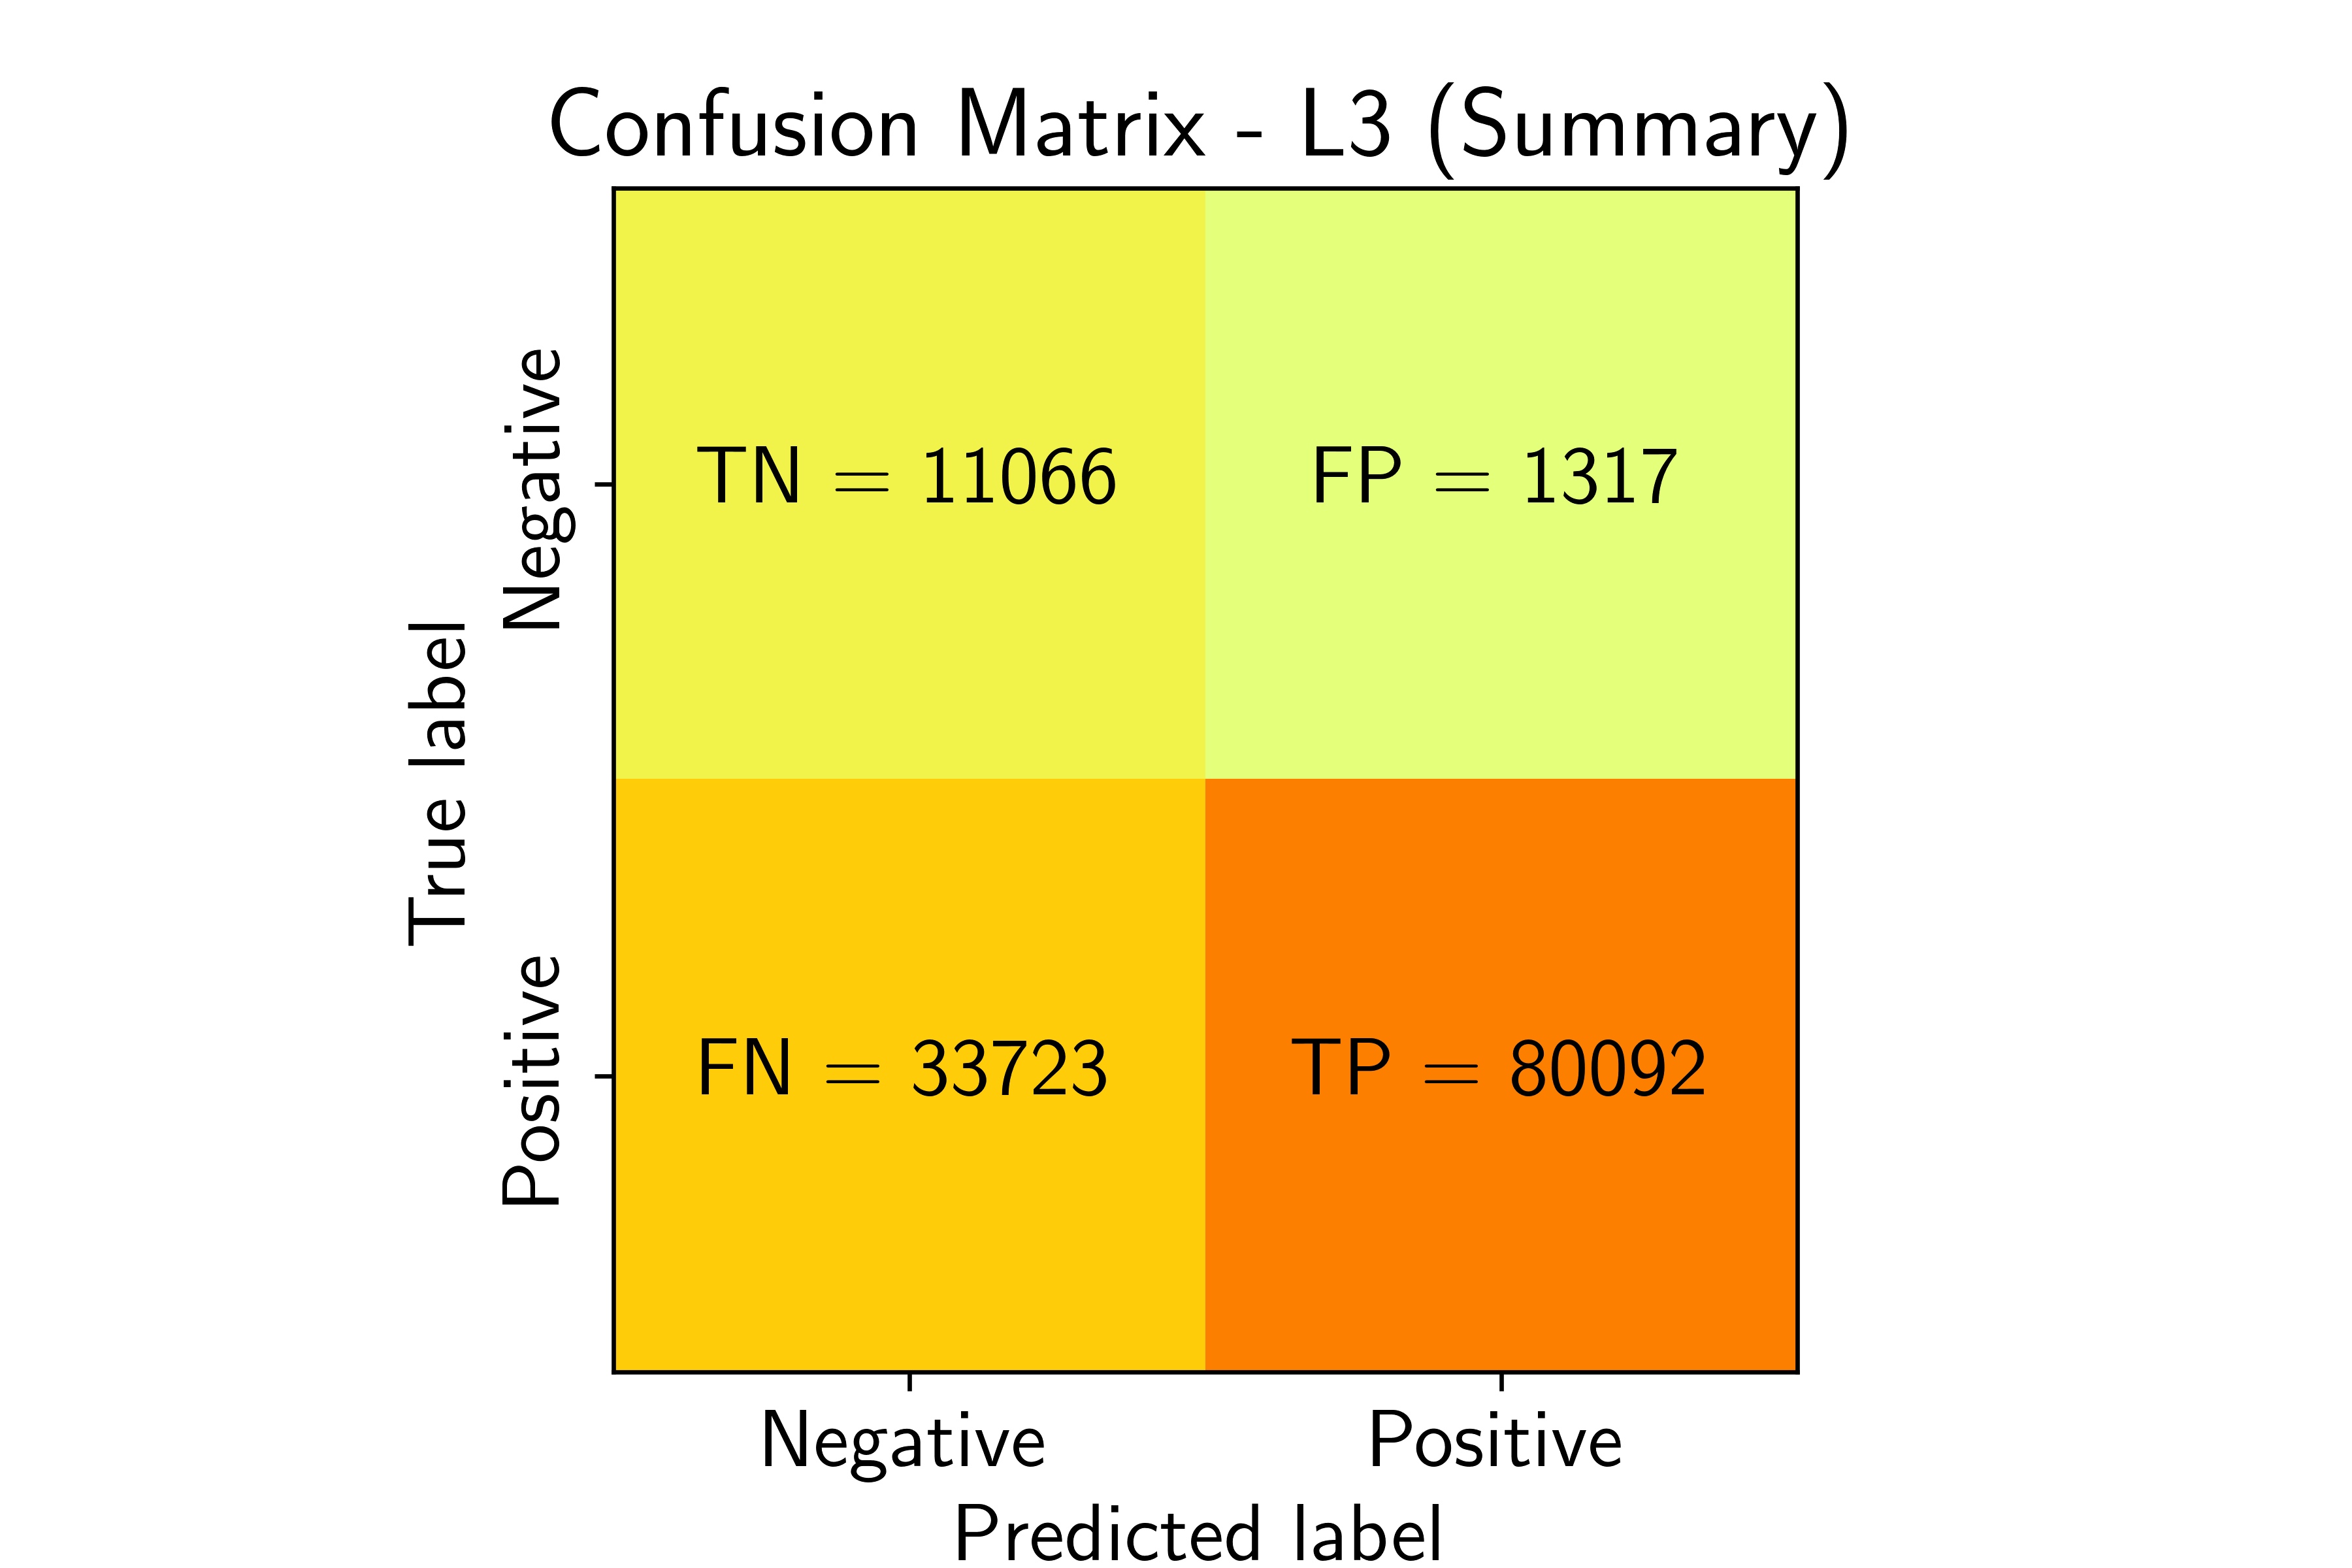
\includegraphics[width=0.48\columnwidth]{figures/Only_Metric/CMonlyL3_SUMMARY.eps}
\end{figure}

Finally, an relevant evaluation on the models that include a handcrafted
feature is necessary: How important is the appended feature for the
model result? The answer can be observed by the feature importance
plots for A2, A3 and L3 in Figure \ref{F8-importance}. Each plot
resembles the importance gain from each feature in the underlying
decision trees that \texttt{XGBoost} uses. Usually, the more bifurcations,
the higher gain a feature has, the more relevance a feature has on
the model prediction itself. All models have the appended feature
as the most important by a good margin, although margin for A3 is
not wide as for A2 or L3.

\begin{figure}[h]
\noindent \begin{centering}
\caption{\label{F8-importance}Importance gain plots for \texttt{Node2Vec}
with each feature}
\par\end{centering}
\begin{centering}
\includegraphics[width=0.48\columnwidth]{figures/ML_Metric/Imp\lyxdot A2\lyxdot All.eps}\includegraphics[width=0.48\columnwidth]{figures/ML_Metric/Imp\lyxdot A3\lyxdot All.eps}
\par\end{centering}
\centering{}\includegraphics[width=0.48\columnwidth]{figures/ML_Metric/Imp\lyxdot L3\lyxdot All.eps}
\end{figure}